
\section{Grundlagen}

Hier erklären was kommt

\subsection{Microservices}

Für den Begriff Microservices existiert keine einheitlich anerkannte Definition. Während Wolff unter Microservices unabhängig, deploybare Module versteht, spricht Newman von kleinen, autonomen Services, die zusammenarbeiten. Cockcroft verwendet den Begriff Microservice gekoppelt mit einem Architekturbegriff: Eine Microservice Architektur sind gekoppelte Services, welche für einen gewissen Kontextbereich zuständig sind. D.h. jeder Service behandelte gewisse, fachliche Aufgaben und kann genau für diese genutzt werden. Eine Vielzahl von solchen Services bildet dann die gesamte Anwendung. \\

Amudsen schreibt dem Microservice an sich die Eigenschaft zu, dass er unabhängig zu anderen Microservices sein muss, d.h. ein Microservice kann losgelöst von anderen geupdated (deployed) werden. Weiter ist ein Microservice wie schon bei Cockcroft für einen gewissen Aufgabenbereich zuständig. Eine Microservice-Architektur ist ein zusammenschluss von miteinander kommunizierenden Microservices. \\

In \textit{Flexible Software Architecture} werden Microservices zu den bisherigen noch weitere, teils technische Eigenschaften zugeschrieben: Microservices sind technologisch unabhängig, d.h. eine Microservice Architektur ist nicht an eine Programmiersprache gebunden. Weiter müssen Microservices einen privaten Datenspeicher haben und sie kommunizieren mit anderen Services über das Netzwerk (z.B. über REST). Ebenfalls werden Microservices verwendet, um große Programme in kleine Teile zu unterteilen. Diese kleine Teile lassen sich automatisch bauen und deployen.  

% Hier beginnt ein neuer Absatz.
%Dies ist der zweite Absatz.
%
% Dann noch ein Unterabschnitt
%\subsection{Ein Unterabschnitt}
%Neuer Text in einem Unterabschnitt.
%
% Und noch ein ganz neuer Abschnitt
%\section{Der nächste Abschnitt}
%Noch mehr Text.

\begin{figure}[ht]
	\centering
	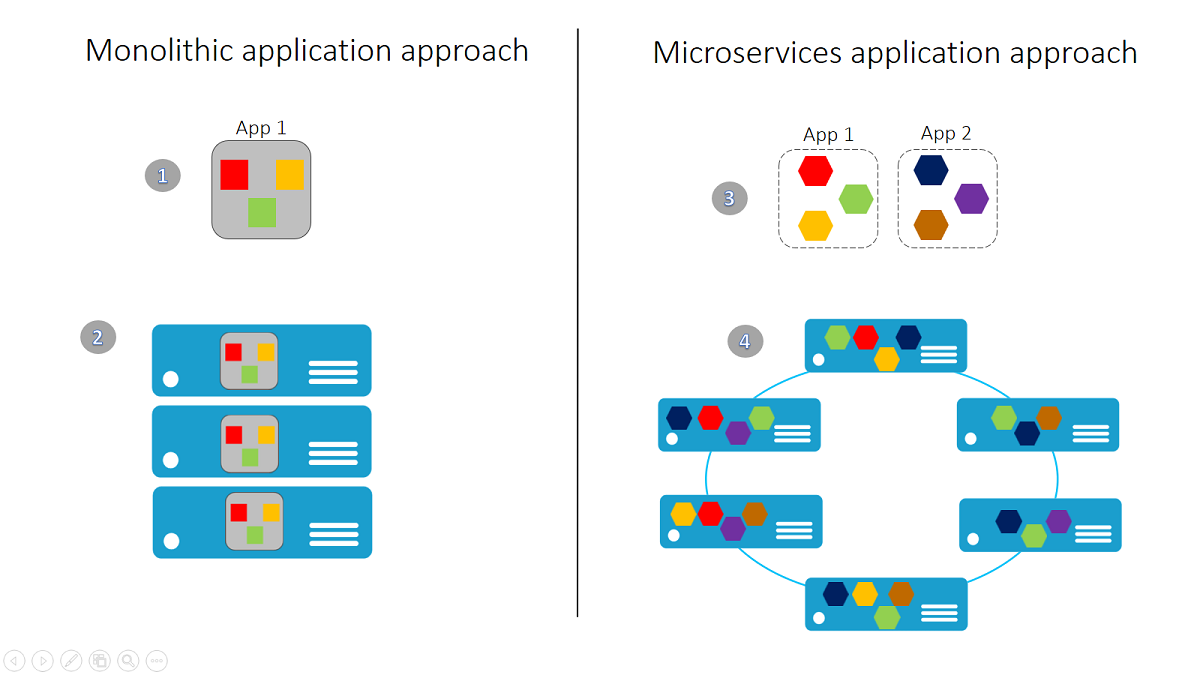
\includegraphics[width=0.9\textwidth]{monolithic_vs_micro}
	\caption{Sie sehen Unterschiede.\cite{irakli2016mic_arc}}
	\label{fig:trigo_funk}
\end{figure}